% Heatmap table of retrieval hit rates on holdout 3 (item level, percent of the 275 questions with a relevant item).
\begin{figure}[htbp]
\centering
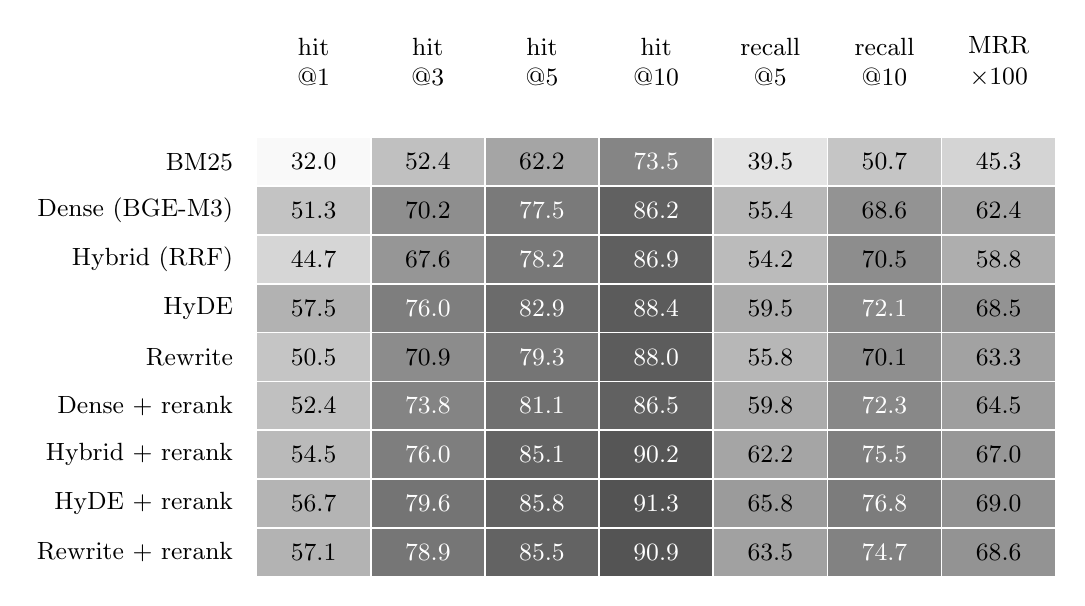
\begin{tikzpicture}[x=1cm,y=1cm,font=\small]
  \def\cw{1.45}
  \def\ch{0.62}
  \def\hc#1#2#3{%
    \pgfmathsetmacro{\sh}{max(0,(#3-30))*1.1}%
    \pgfmathparse{#3>=72?1:0}%
    \ifnum\pgfmathresult=1 \def\tc{white}\else\def\tc{black}\fi
    \node[fill=black!\sh,text=\tc,minimum width=\cw cm,minimum height=\ch cm,inner sep=0pt,draw=white,line width=.6pt] at ({3.2+#1*\cw},{-#2*\ch}) {#3};%
  }
  \foreach \c/\lab in {0/{hit\\@1},1/{hit\\@3},2/{hit\\@5},3/{hit\\@10},4/{recall\\@5},5/{recall\\@10},6/{MRR\\$\times$100}} {
    \node[align=center] at ({3.2+\c*\cw},0.65) {\lab};
  }
  \foreach \r/\name/\a/\b/\c/\d/\f/\g/\e in {
    1/{BM25}/32.0/52.4/62.2/73.5/39.5/50.7/45.3,
    2/{Dense (BGE-M3)}/51.3/70.2/77.5/86.2/55.4/68.6/62.4,
    3/{Hybrid (RRF)}/44.7/67.6/78.2/86.9/54.2/70.5/58.8,
    4/{HyDE}/57.5/76.0/82.9/88.4/59.5/72.1/68.5,
    5/{Rewrite}/50.5/70.9/79.3/88.0/55.8/70.1/63.3,
    6/{Dense + rerank}/52.4/73.8/81.1/86.5/59.8/72.3/64.5,
    7/{Hybrid + rerank}/54.5/76.0/85.1/90.2/62.2/75.5/67.0,
    8/{HyDE + rerank}/56.7/79.6/85.8/91.3/65.8/76.8/69.0,
    9/{Rewrite + rerank}/57.1/78.9/85.5/90.9/63.5/74.7/68.6} {
    \node[left] at (2.3,-\r*\ch) {\name};
    \hc{0}{\r}{\a}\hc{1}{\r}{\b}\hc{2}{\r}{\c}\hc{3}{\r}{\d}\hc{4}{\r}{\f}\hc{5}{\r}{\g}\hc{6}{\r}{\e}
  }
\end{tikzpicture}
\caption[Retrieval methods on holdout 3, measured at the item level (a chunk counts for its document)]{Retrieval methods on holdout 3, measured at the item level (a chunk counts for its document). The hit@$k$ cells give the percentage of the 275 emails with a relevant item for which a relevant item appears in the top $k$. The recall@$k$ cells give the percentage of an email's relevant items that appear in the top $k$, averaged over the 275 emails. The last column is the mean reciprocal rank multiplied by 100. Darker cells are higher values. The 4 bottom rows add the cross-encoder reranker on the top 30 candidates.}
\label{fig:recall-heatmap}
\end{figure}
